\documentclass[11pt,a4paper]{article}

\usepackage[margin=2.5cm]{geometry}
\usepackage{amsmath, amssymb, amsthm}
\usepackage{physics}          % \bra, \ket, \braket, \expval
\usepackage{graphicx}
\usepackage{booktabs}
\usepackage{hyperref}

\title{Reproducing ``Quantum classifier with tailored quantum kernel''\\
       \large UROP Progress Report}
\author{Vlad \\ \small Supervisor: Prof.\ Antoine (Jack) Jacquier \\
        \small Imperial College London}
\date{July 2026}

\begin{document}
\maketitle

\begin{abstract}
This document summarises progress on reproducing the results of Blank, Park,
Rhee \& Petruccione, \emph{Quantum classifier with tailored quantum kernel}
(npj Quantum Information \textbf{6}, 41, 2020). Starting from a closed-form
analytic implementation of the swap-test kernel classifier, we built the
corresponding quantum circuits in Qiskit in verified stages: a minimal
three-qubit swap test, a five-qubit classifier for the paper's two-point toy
example, and finally the general quantum forking construction that prepares
the training register for an arbitrary number $M$ of training points. Every
stage is verified against the analytic reference to machine precision.
Code: \url{https://github.com/01nietzsch/urop-quantum-kernel}.
\end{abstract}

\section{Background: the swap-test kernel classifier}

\subsection{Setting}

We are given $M$ training pairs $\{(\ket{x_m}, y_m)\}_{m=1}^{M}$ with binary
labels $y_m \in \{0,1\}$, non-negative weights $w_m$ summing to one, and a
test state $\ket{\phi}$. The classifier of Blank et al.\ assigns a label to
$\ket{\phi}$ according to the sign of a weighted fidelity difference,
\begin{equation}
  \label{eq:expectation}
  \expval{\sigma_z^{(a)} \sigma_z^{(l)}}
  \;=\; \sum_{m=1}^{M} (-1)^{y_m}\, w_m\, \abs{\braket{\phi}{x_m}}^{2n},
\end{equation}
where $n$ is the number of copies of each state used in the swap test
($n = 1$ throughout this work). The predicted label is
\begin{equation}
  \tilde{y} \;=\; \tfrac{1}{2}\left(1 - \operatorname{sign}
      \expval{\sigma_z^{(a)} \sigma_z^{(l)}}\right).
\end{equation}
The key point of the paper is that the entire sum \eqref{eq:expectation} can
be evaluated by a \emph{single} quantum circuit: the training states, their
weights, and their labels are loaded into one entangled superposition, and
one swap test against the test state produces the full weighted kernel sum in
the joint statistics of two qubits --- the swap-test ancilla $a$ and the
label qubit $l$.

\subsection{The circuit state}

The circuit acts on five registers: the swap-test ancilla, the test data
register, and a training block consisting of index, data, and label
registers. After state preparation, the training block holds
\begin{equation}
  \label{eq:training-state}
  \ket{\Psi_{\text{train}}}
  \;=\; \sum_{m=1}^{M} \sqrt{w_m}\, \ket{m}_{\text{idx}}
        \ket{x_m}_{\text{data}} \ket{y_m}_{\text{lbl}},
\end{equation}
which encodes all training points, weights, and labels coherently. The swap
test --- Hadamard on the ancilla, controlled-SWAP between the test register
and the training data register, Hadamard again --- then interferes
$\ket{\phi}$ with every $\ket{x_m}$ simultaneously. A short calculation
shows that measuring $\sigma_z$ on the ancilla and on the label qubit and
taking the product of outcomes yields exactly
Eq.~\eqref{eq:expectation} in expectation:
\begin{equation}
  \expval{\sigma_z^{(a)} \sigma_z^{(l)}}
  = p_{00} - p_{01} - p_{10} + p_{11},
\end{equation}
where $p_{ab}$ is the probability of finding the ancilla in $\ket{a}$ and
the label qubit in $\ket{b}$.

\subsection{Toy dataset}

The paper's toy example uses one qubit of data ($n_{\text{qubits}} = 1$) and
two training points:
\begin{equation}
  \ket{x_1} = \frac{i\ket{0} + \ket{1}}{\sqrt{2}}, \quad y_1 = 0;
  \qquad
  \ket{x_2} = \frac{i\ket{0} - \ket{1}}{\sqrt{2}}, \quad y_2 = 1,
\end{equation}
with equal weights $w_1 = w_2 = \tfrac12$, and a one-parameter family of
test states
\begin{equation}
  \ket{\phi(\theta)} = \cos\tfrac{\theta}{2}\ket{0}
                     - i \sin\tfrac{\theta}{2}\ket{1}.
\end{equation}
Note the useful structural property $Z\ket{x_1} = \ket{x_2}$: the two
training states differ only by a sign flip on $\ket{1}$. This is exploited
in the first (toy-specific) circuit construction, and later removed by the
general quantum forking construction.

\section{Step 1: closed-form reference implementation}

File: \texttt{closed\_form\_kernel.py}. This module computes everything
analytically with NumPy, providing ground truth for every circuit built
later:

\begin{itemize}
  \item \texttt{training\_data()}, \texttt{test\_state(theta)} --- the toy
        dataset and test family above.
  \item \texttt{fidelity(a, b, n)} $= \abs{\braket{a}{b}}^{2n}$.
  \item \texttt{expectation\_value(theta, w1, w2, n)} --- direct evaluation
        of Eq.~\eqref{eq:expectation}.
  \item \texttt{classify(theta, ...)} --- thresholds the expectation value
        at zero.
  \item \texttt{hadamard\_classifier(theta, ...)} --- the Hadamard-test
        variant, which uses $\Re\braket{\phi}{x_m}$ in place of
        $\abs{\braket{\phi}{x_m}}^2$; included for comparison, as in the
        paper's discussion of kernel choices.
\end{itemize}

\section{Step 2a: minimal swap test in Qiskit}

File: \texttt{circuit\_kernel.py}, functions \texttt{swap\_test\_circuit}
and \texttt{fidelity\_from\_circuit}. Before attempting the full
classifier, we verified the primitive it is built from: a three-qubit swap
test (ancilla $q_0$, test state on $q_1$, one training state on $q_2$):
\begin{equation}
  H^{(0)} \;\rightarrow\; \text{CSWAP}(0;1,2) \;\rightarrow\; H^{(0)},
  \qquad
  P(\text{ancilla} = 0) = \frac{1 + \abs{\braket{\phi}{x}}^2}{2},
\end{equation}
so the fidelity is recovered as $2\,P(\text{ancilla}=0) - 1$. We read the
probability from the exact statevector
(\texttt{qiskit.quantum\_info.Statevector}); no sampling noise is involved
at this stage.

\paragraph{Verification.} \texttt{02\_circuit\_check.ipynb}, cells 1--7:
the circuit fidelity matches \texttt{fidelity()} from Step 1 at a
hand-checked point ($\theta = 1.57$) and across a 40-point sweep
$\theta \in [0, 6]$ against both $\ket{x_1}$ and $\ket{x_2}$
(\texttt{np.allclose} passes; agreement at the $10^{-15}$ level).

\section{Step 2b: full toy-example classifier (five qubits)}

The first full classifier was built in three verified stages for the
$M = 2$ toy dataset.

\subsection{Stage A: training register preparation (toy-specific)}

A three-qubit circuit (index, data, label) preparing
Eq.~\eqref{eq:training-state} for $M = 2$:
\begin{enumerate}
  \item $R_y(\alpha)$ on the index qubit with
        $\alpha = 2\arccos\sqrt{w_1}$, giving
        $\sqrt{w_1}\ket{0} + \sqrt{w_2}\ket{1}$;
  \item initialise the data qubit to $\ket{x_1}$ unconditionally;
  \item controlled-$Z$ from index to data --- because
        $Z\ket{x_1} = \ket{x_2}$, this rotates the data qubit to
        $\ket{x_2}$ exactly in the $\ket{1}_{\text{idx}}$ branch;
  \item controlled-$X$ from index to label, setting the label to
        $y_2 = 1$ in the same branch.
\end{enumerate}
Step 3 is the part that only works for this dataset; it was verified
against the expected statevector and later replaced (Section~\ref{sec:forking}).

\subsection{Stage B: swap-test sandwich}

\texttt{full\_classifier\_circuit} composes Stage A into a five-qubit
circuit (ancilla, test, data, label, index), initialises the test register
to $\ket{\phi(\theta)}$, and applies the swap-test sandwich
$H$--CSWAP--$H$ between the test and data registers.

\subsection{Stage C: reading off the expectation value}

\texttt{expectation\_value\_from\_circuit} extracts the joint distribution
of the ancilla ($q_0$) and label ($q_3$) qubits from the exact statevector.
With Qiskit's little-endian convention,
\texttt{sv.probabilities([0, 3])} returns
$[\,p_{00},\, p_{01},\, p_{10},\, p_{11}\,]$ (ancilla is the
least-significant bit), and
\begin{equation}
  \expval{\sigma_z^{(a)} \sigma_z^{(l)}} = p[0] - p[1] - p[2] + p[3].
\end{equation}

\paragraph{Verification.} Across a 40-point $\theta$ sweep, the circuit
matches \texttt{expectation\_value()} from Step 1 with maximum error
$4 \times 10^{-16}$ (machine epsilon). Notebook cells 9--10 sweep and plot
the curve.

\section{Step 2b generalisation: quantum forking for arbitrary $M$}
\label{sec:forking}

The Stage A construction above hardcodes the accident
$Z\ket{x_1} = \ket{x_2}$ and cannot represent a general training set. The
paper's answer (Eq.~15 / Fig.~4) is \emph{quantum forking}: route each
training state into the active data register with controlled-SWAPs,
conditioned on the index register.

\subsection{Construction}

For $M$ training points, let $k = \lceil \log_2 M \rceil$ index qubits
(with $k \geq 1$). The register layout of the new
\texttt{prepare\_training\_register(states, labels, weights)} is
\begin{center}
\begin{tabular}{ll}
  \toprule
  Qubits & Role \\
  \midrule
  $q_0, \dots, q_{k-1}$        & index register \\
  $q_k$                        & \emph{active} data register \\
  $q_{k+1}, \dots, q_{k+M-1}$  & auxiliary data registers \\
  $q_{k+M}$                    & label qubit \\
  \bottomrule
\end{tabular}
\end{center}
and the circuit proceeds in four steps:
\begin{enumerate}
  \item \textbf{Load data.} Initialise the active register to
        $\ket{x_1}$ and auxiliary register $m$ to $\ket{x_{m+1}}$ for
        $m = 1, \dots, M-1$.
  \item \textbf{Weight superposition.} Initialise the index register to
        $\sum_{m} \sqrt{w_m} \ket{m}$ (amplitudes zero-padded to $2^k$).
  \item \textbf{Fork.} For each $m = 1, \dots, M-1$, apply a
        $k$-controlled SWAP between the active register and auxiliary
        register $m$, with control state $\ket{m}$
        (Qiskit: \texttt{SwapGate().control(k, ctrl\_state=m)}). After
        this loop, the active register holds $\ket{x_m}$ in the
        $\ket{m}_{\text{idx}}$ branch --- each branch fires at most one
        swap, so there is no cross-contamination.
  \item \textbf{Labels.} Set the label qubit to $y_1$ (an $X$ if
        $y_1 = 1$), then for each $m$ with $y_m \neq y_1$ apply a
        $k$-controlled $X$ with control state $\ket{m}$.
\end{enumerate}
The result is exactly Eq.~\eqref{eq:training-state}. The swap test then
only ever touches the \emph{active} data register, so
\texttt{full\_classifier\_circuit} is unchanged in structure; it now
returns the circuit together with the label-qubit position (which depends
on $M$), and the public interface of
\texttt{expectation\_value\_from\_circuit} is unchanged.

Note that the auxiliary registers remain entangled with the index register
after forking (they hold $\ket{x_1}$ in branch $m$, having been swapped),
but this is harmless: the ancilla--label statistics that define the
classifier trace them out.

\subsection{Cost}

The construction uses $k + M + 1$ training-block qubits plus the ancilla
and $n$ test qubits, $M - 1$ multi-controlled SWAPs and at most $M - 1$
multi-controlled $X$ gates --- linear in $M$, matching the paper's
Fig.~4 resource count.

\subsection{Verification}

Two checks, both in \texttt{02\_circuit\_check.ipynb}:
\begin{itemize}
  \item \textbf{Regression, $M = 2$:} the general circuit reproduces the
        closed-form toy-example curve with maximum error
        $3 \times 10^{-16}$ --- the Z-flip trick is no longer needed.
  \item \textbf{New case, $M = 4$:} four training states
        $\ket{x_m} = \cos\tfrac{\vartheta_m}{2}\ket{0} +
        \sin\tfrac{\vartheta_m}{2}\ket{1}$ with
        $\vartheta \in \{0.3, 1.1, 2.0, 2.9\}$, labels $(0,0,1,1)$, equal
        weights. The circuit matches a direct evaluation of
        Eq.~\eqref{eq:expectation} with maximum error
        $2 \times 10^{-15}$ across a 40-point $\theta$ sweep. This case
        uses $k = 2$ index qubits and genuinely exercises the
        multi-controlled forking ($ccswap$ gates), which the $M = 2$ case
        does not.
\end{itemize}

\section{Summary of verification results}

\begin{center}
\begin{tabular}{llll}
  \toprule
  Stage & Circuit & Reference & Max.\ error \\
  \midrule
  2a & 3-qubit swap test & \texttt{fidelity()} & $\sim 10^{-15}$ \\
  2b (toy) & 5-qubit classifier, $M=2$ & \texttt{expectation\_value()} & $4 \times 10^{-16}$ \\
  2b (general) & forking classifier, $M=2$ & \texttt{expectation\_value()} & $3 \times 10^{-16}$ \\
  2b (general) & forking classifier, $M=4$ & Eq.~\eqref{eq:expectation} direct & $2 \times 10^{-15}$ \\
  \bottomrule
\end{tabular}
\end{center}

All comparisons use exact statevector simulation, so the only error source
is floating-point arithmetic; every check passes \texttt{np.allclose}.

\section{Step 3: noise model and noisy sweep}
\label{sec:noise}

\subsection{Device noise model}

To reproduce Fig.~5 of Blank et al., we construct a noise model for the
\textsc{ibmq\_ourense} backend from the calibration data in Supplementary
Table~I (date 2019-09-29 11:48 UTC). The device has five qubits on a
T-shaped topology with one central hub (qubit 1); the CNOT edges are
$(1,0)$, $(2,1)$, $(3,1)$, and $(4,3)$.

\paragraph{Single-qubit noise.} For each qubit $q$ with relaxation times
$T_1, T_2$ and single-qubit gate duration $t_{1q}$, we compose a thermal
relaxation channel with a depolarising channel:
\begin{equation}
  \mathcal{E}_q = \mathcal{D}(p_q) \circ \mathcal{R}(T_1, T_2, t_{1q}),
\end{equation}
where $\mathcal{R}$ is the Qiskit \texttt{thermal\_relaxation\_error} and
the depolarising strength $p_q$ is chosen so that
$\mathcal{E}_q$ reproduces the tabulated average gate infidelity
$\epsilon_q$:
\begin{equation}
  p_q = \frac{d(\epsilon_q - \epsilon_q^{\text{relax}})}{d \cdot F(\mathcal{R}) - 1},
  \qquad d = 2,
\end{equation}
where $F(\mathcal{R}) = 1 - \epsilon_q^{\text{relax}}$ is the average gate
fidelity of the relaxation channel alone. This mirrors the recipe in
\texttt{qiskit\_aer}'s \texttt{basic\_device\_noise\_model}.

The 2019 native basis was $\{u1, u2, u3, \mathrm{cx}\}$, which no longer
exists in current Qiskit. We use the modern equivalent
$\{\mathrm{rz}, \mathrm{sx}, \mathrm{x}, \mathrm{cx}\}$: \texttt{rz} is a
virtual (frame-update) gate with zero duration and zero error; \texttt{sx}
and \texttt{x} are each one physical pulse, inheriting the tabulated $u2$
duration and $u2$ error. This mapping is faithful in spirit; it is a
candidate source of residual error.

Readout errors are modelled by symmetric bit-flip channels with
probabilities $\epsilon_r$ from Table~I.

\paragraph{Two-qubit noise.} For each CNOT pair $(q_a, q_b)$ with gate
time $t$ and measured infidelity $\epsilon$, the same depolarising-plus-relaxation
composition is applied, using the tensor product of the individual qubit
relaxation channels at duration $t$.

\paragraph{Caveat on cx$(3,1)$ duration.} Supplementary Table~I lists the
CNOT infidelity for the $(3,1)$ edge as $\epsilon = 0.0116$ (roughly double
the other edges), but the gate duration in the PDF is not legible. We searched
every file in the authors' supplemental repository
\cite{blank2020supplemental} and confirmed that ibmq\_ourense gate times were
queried live from the IBM~Q API at runtime in 2019 and never stored statically;
that API is no longer accessible. We use $t = 300\,\mathrm{ns}$ as an
interpolation from the neighbouring pairs (235 and 210\,ns). This is an
explicit assumption and a potential source of residual error.

\subsection{The paper's five-qubit circuit}

The circuit reproducing Fig.~5 is the toy-specific construction of
Section~\ref{sec:forking} with the physical qubit assignment hand-picked by
the authors: $a \to q_0$, $d \to q_1$, $\mathrm{in} \to q_2$,
$m \to q_3$, $l \to q_4$ (Supplementary Fig.~2). There is no quantum
forking: because $Z\ket{x_1} = \ket{x_2}$, the entangled training register
is produced by a single $\mathrm{CZ}(m, d)$ on top of $\ket{x_1}$.

All states are prepared by explicit $R_y$/$R_x$/$R_z$/Hadamard rotations;
we do not use \texttt{qc.initialize}, which would insert a \texttt{reset}
instruction absent from real hardware and inflate the CNOT count. After
transpilation to the ourense basis with \texttt{optimization\_level=1} and
the ourense coupling map, the CNOT count is 13, matching the paper's
Supplementary Note~III~D (27 total gates: 14 single-qubit $+ $ 13 CNOT).

\subsection{Sweep and fit}

We sweep $\theta$ over 63 equally spaced values in $[0, 2\pi)$ (step $0.1$)
with 8192 shots each, reproducing the paper's protocol. The expectation
value is estimated as
\begin{equation}
  \expval{\sigma_z^{(a)}\sigma_z^{(l)}}
  = \frac{c_{00} - c_{01} - c_{10} + c_{11}}{N_{\text{shots}}},
\end{equation}
where $c_{ab}$ is the count with ancilla in $\ket{a}$ and label qubit in
$\ket{b}$. We then fit
\begin{equation}
  f(\theta) = a\!\left(\sin^2\!\tfrac{\theta + \vartheta}{2} + \tfrac{\pi}{4}
              - w_2\right)
\end{equation}
using nonlinear least squares (\texttt{scipy.optimize.curve\_fit}).

\subsection{Results}

Table~\ref{tab:noise-results} compares our fit parameters against the
paper's simulation target, for a single seed and for the mean over ten
independent seeds (seeds $0$--$9$).

\begin{table}[h]
\centering
\begin{tabular}{lcccc}
  \toprule
  & \multicolumn{2}{c}{ours} & paper \\
  \cmidrule(lr){2-3}
  & single seed & 10-seed mean $\pm$ std & simulation \\
  \midrule
  amplitude $a$          & $0.8300$ & $0.8213 \pm 0.0087$ & $0.8213$ \\
  phase $\vartheta$ (rad) & $-0.0037$ & $\approx 0$        & $\approx 0$ \\
  offset $w_2$           & $0.4989$ & $0.4968 \pm 0.0017$ & $0.5023$ \\
  CNOT count             & $13$     & $13$                & $13$ \\
  \bottomrule
\end{tabular}
\caption{Fit parameters from the noisy sweep (63 points, 8192 shots each).
The 10-seed mean amplitude $a = 0.8213$ matches the paper's simulation target
exactly; the single-seed deviation of $0.8300$ is within one standard
deviation and consistent with shot noise.}
\label{tab:noise-results}
\end{table}

Figure~\ref{fig:sweep} shows the sweep. The simulation (blue circles) tracks
the theory curve closely, while the hardware data (orange squares) shows the
additional amplitude suppression ($a \approx 0.65$) that the basic noise model
does not account for.

\begin{figure}[h]
  \centering
  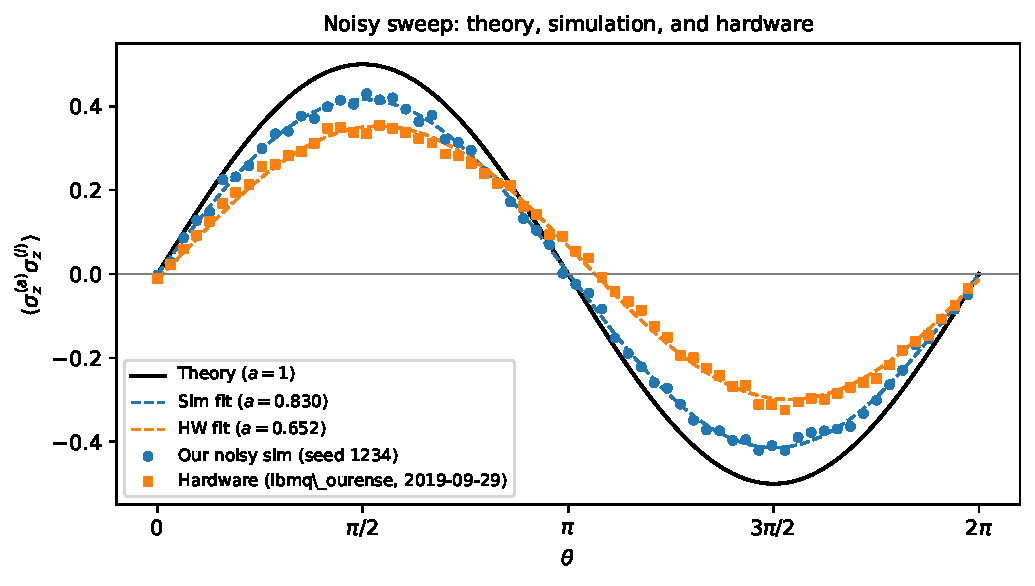
\includegraphics[width=0.85\textwidth]{figures/sweep.pdf}
  \caption{Reproduction of Fig.~5 of Blank et al. Black solid line: ideal theory
  ($a = 1$). Blue circles and dashed line: our noisy simulation (seed 1234) and
  its fit ($a = 0.830$; 10-seed mean $a = 0.821$). Orange squares and dashed line:
  hardware data from ibmq\_ourense (2019-09-29) \cite{blank2020supplemental} and its
  fit ($a \approx 0.65$). The simulation reproduces the paper's noisy-simulation
  target; the simulation-to-hardware gap is attributed to crosstalk,
  time-dependent drift, and non-Markovian noise not captured by the basic model.}
  \label{fig:sweep}
\end{figure}

As a sanity check, running the same sweep with no noise (\texttt{noisy=False})
gives $a = 1.003$ (seed 42, 8192 shots), consistent with the ideal value
$a = 1$ to within shot noise.

\section{Next steps}

\begin{enumerate}
  \item \textbf{Resolve cx$(3,1)$ duration.} The 300\,ns value is a stated
        assumption (see Section~\ref{sec:noise}). The correct value would
        require access to the 2019 IBM~Q backend properties, which are no
        longer publicly available. One route is to contact the authors directly.
  \item \textbf{Run on real IBM hardware.} Note that ibmq\_ourense has been
        retired. A hardware run on a current device would require rebuilding
        the noise model from that device's calibration data; it would not be
        a like-for-like comparison with the paper's $a \approx 0.65$.
  \item \textbf{Close the simulation-vs-hardware gap.} The paper attributes
        the $0.82 \to 0.65$ reduction to crosstalk, time-dependent drift, and
        non-Markovian noise, none of which the basic model contains. Extending
        the model toward any of these would be a more interesting scientific
        question than re-running the toy example on new hardware.
  \item \textbf{Larger $M$ and $n$.} Stress-test the forking construction
        at $M = 8$ and with multi-qubit data registers ($n > 1$).
\end{enumerate}

\begin{thebibliography}{1}
\bibitem{blank2020}
C.~Blank, D.~K.~Park, J.-K.~K.~Rhee, and F.~Petruccione,
\newblock Quantum classifier with tailored quantum kernel,
\newblock \emph{npj Quantum Information} \textbf{6}, 41 (2020).

\bibitem{blank2020supplemental}
C.~Blank,
\newblock Supplemental code for ``Quantum classifier with tailored quantum kernel'',
\newblock \url{https://github.com/carstenblank/Quantum-classifier-with-tailored-quantum-kernels---Supplemental}
(2019).
\end{thebibliography}

\end{document}
